%\documentclass[12pt,letterpaper,onecolumn]{article}
%\documentclass[11pt,letterpaper,onecolumn]{article}
\documentclass[10pt,letterpaper,onecolumn]{article}
%\documentclass[12pt,letterpaper,twocolumn]{article}
%\documentclass[11pt,letterpaper,twocolumn]{article}
%\documentclass[10pt,letterpaper,twocolumn]{article}


%\usepackage{amsmath}
\usepackage{subcaption}
%\usepackage{graphics}
\usepackage{graphicx} %more modern version of graphics
%\graphicspath{{path-to-folder-containing-necessary-graphics}{other folder as necessary}}



\begin{document}

\title{\Large\bf Measuring the Half Life of Ba-137 Using a Scintillator Detector}
\author{
 Akhil Deshpande \\*
  \\*
 PHY 353L Modern Laboratory \\*
 Department of Physics \\*
 The University of Texas at Austin \\*
 Austin, TX 78712, USA
}
\date{September 15, 2023}



\maketitle
\begin{abstract}

  In this study, we explored the specifics of radioactive half life. We used a photomultiplier
  tube as well as a scinitillator detector to measure the half life of a sample of Ba-137.
  The experimental setup comprised an array of sophisticated equipment, 
  including an ORTEC model 113 scintillation preamplifier, model 672 spectroscopy 
  amplifier, and a model 553 timing single-channel analyzer (SCA). 
  These were supplemented by an oscilloscope and a National 
  Instruments DAQ interfacing with NI LabView software for precise data capture.
  We determined the half life to be within the accepted range for a sample of Ba-137.
  Our observation was that the average half lifes of samples of Ba-137 to be 
  $163.1 \pm 8.5$ seconds.

 

\end{abstract}
\section{Introduction}
\subsection{Physics Motivation}
In this study, we investigate the principles of radioactive decay 
law by monitoring the activity levels of a radioactive isotope, Ba-137m, 
over a period of time. Fundamentally, radioactivity involves the transition 
of unstable atomic nuclei to a more stable state through the release of alpha, 
beta, or gamma radiation. This transition occurs at random, yet maintains a consistent 
probability of occurrence over time, thereby forming an exponential decay curve in both
 activity and the number of nuclei present within a given sample.

It is noteworthy that this process gives rise to either new elements or new 
isotopes of the existing element. Additionally, the 'm' denotation in an isotope's 
name, such as in Ba-137m, signifies that the isotope exists in an elevated energy state, 
as referenced in [1]. 
The aims of this study are twofold: 
firstly, to illustrate the exponential nature of radioactive decay, 
and secondly, to ascertain the radioactive half-life of Ba-137m.
\subsection{Historical context}
By the year 1902, Ernest Rutherford had delineated radiation into three 
distinct categories: alpha, beta, and gamma radiation, as documented in [2]. 
Alpha radiation encompasses helium-4 nuclei, which are produced during the alpha 
decay of a nucleus. Beta particles, on the other hand, are comprised of electrons or 
positrons that are released when a neutron decays into a proton or the inverse process 
takes place. Conversely, gamma rays are high-energy photons that are released when a 
nucleus transitions from a high to a lower energy state. Rutherford discovered that gamma
 rays have a significantly higher penetration capacity through various materials 
 compared to alpha and beta particles [2], a characteristic that facilitates the
  differentiation of gamma decays from other types in detectors.

The initial scintillation detector, termed a spinthariscope, was devised by Sir 
William Crookes in 1903. This instrument employed a zinc sulfide (ZnS) screen 
combined with a microscope, enabling the visualization of light flashes whenever 
alpha particles struck the screen. A decade later, in 1910, Ernest Marsden and 
Hans Geiger utilized the spinthariscope to conduct the inaugural coincidence experiment. 
This involved placing a radioactive gas between two screens and relying on human 
observers equipped with microscopes on each flank of the double-screen to tally the 
perceived flashes. Despite this innovation, the method proved to be somewhat 
inadequate as human observation was relatively slow and prone to errors, leading to 
the temporary abandonment of the scintillation counter.

Nonetheless, in 1944, scintillators made a comeback, this time incorporating 
photomultipliers to supplant human observation, thereby enhancing accuracy and 
reliability. Presently, two prevalent varieties of scintillators are in widespread use: 
sodium iodide (NaI) crystals, which are infused with a trace quantity of thallium and 
primarily employed for gamma ray detection, and plastic scintillators, which are 
predominantly utilized in detecting charged particles, as noted in [3].





\section{Theoretical background}
\subsection{Statistics of Radioactive Decay}
The number of counts, N, models how many gamma rays are detected by the SCA, and counted
by our apparatus. Because N is a counting variable, it is subject to a Poisson distribution.
In a time interval t, the probability
that N counts observed, P (N), is:
$$
P(N) = \frac{\bar{N}^N e^{-\bar{N}}}{N!}
$$
Here, \( \bar{N} \) represents the mean 
count over the same time interval for a given sample size.
 It is important to note that \( P(N) \) exemplifies a Poisson distribution, 
 which tends to a Gaussian distribution with a peak at \( \bar{N} \) 
 and a standard deviation of \( \bar{N}^{1/2} \) for large values of \( N \).

\section{Experimental setup}
\subsection{Apparatus}
When a gamma ray penetrates the crystal in a scintillator detector, 
it undergoes interactions with the confined 
electrons via three primary pathways: the photoelectric effect, Compton scattering,
and electron-positron pair creation. However, since the latter only occurs for gamma 
rays with energies exceeding 1.02 MeV and the rays we are detecting are at 662 keV, 
we can disregard this mechanism. At energies below 100 keV, the photoelectric effect 
is prevalent, while Compton scattering is the dominant process between 100 keV and 1 MeV.

In the context of the photoelectric effect, the incoming gamma ray is absorbed by an 
electron in the crystal, imparting it with an energy \(E_e = E_\gamma - E_b\), 
where \(E_\gamma\) is the gamma ray's energy and \(E_b\) is the binding energy of the 
electron before being displaced by the photon. This energized electron subsequently 
collides with another electron in the crystal, initiating a series of interactions with 
other electrons, thereby creating a cascade within the crystal. Ultimately, these 
electrons revert to a lower energy state within the crystal, each emitting a low-energy 
photon that progresses towards the PMT. This generates a significant peak in the
crystal's spectrum, proportional to \(E_e\), with the peak width \(\Delta E\) being 
dependent on the photon count produced by the gamma ray, which diminishes as 
\(E_\gamma\) augments.

During Compton scattering, the photon interacts with an electron, causing it to 
recoil with an energy dependent on the scattering angle of the photons. 
These photons then reach the PMT's photocathode, releasing electrons which are 
subsequently accelerated and concentrated onto the first dynode. Here, each electron
 generates 2-5 secondary electrons, a process that repeats across up to 14 amplification 
 stages. This amplification is facilitated by progressively increasing the voltage at
  each dynode, culminating in a discernible current pulse generated from the initial 
  few photons. This mechanism necessitates a substantial voltage supply for the PMT,
   with our experiment utilizing a 750 V supply, although PMTs generally require 
   between 1000-2000 V.

Our experimental setup also incorporates other key components including an ORTEC 
model 113 scintillation preamplifier, model 672 spectroscopy amplifier, and a model 
553 timing single-channel analyzer (SCA), complemented by an oscilloscope and a
 National Instruments DAQ connected to a computer for data recording.

I will now detail the function and configuration of each element in our setup. 
Initially, the 113 preamplifier transforms the current pulse generated at the PMT's 
anode into a voltage pulse, leveraging multiple capacitors. 
This includes a variable capacitor controlled by a front panel dial, allowing us to 
modify the voltage pulse amplitude, set at 200 pF in our case. The 672 amplifier, 
receiving signals from the preamplifier, enhances the signal for compatibility with 
both single and multi-channel pulse height analyzers It offers a variable gain, set at 
200 for our experiment, and facilitates signal shaping with adjustable shaping time. 
Following the 672 manual's recommendation for NaI scintillators, we used a shaping 
time of 1 microsecond. Moreover, we utilized the amplifier's bipolar output to distinguish 
the PMT's output signal from oscilloscope noise.

The 553 timing SCA processes both unipolar and bipolar input pulses, assessing the
amplitude of each pulse and producing a corresponding rectangular output pulse on the 
input pulse's falling edge. This equipment enables the establishment of lower and upper 
thresholds to filter voltage pulses within a specified amplitude range. After meticulous 
adjustment using the oscilloscope, we determined optimal thresholds of 0.8 V (lower) and
approximately 3.5 V (upper).

Lastly, the National Instruments DAQ interfaces with the NI LabView software, 
monitoring the pulse counts outputted by the SCA with software furnished by the 
instructor. Leveraging the DAQ's in-built timer, we achieved high precision in timing, 
configuring the software to register pulse counts in intervals of one second.

\subsection{Data Collection}

Initially, we had to calibrate our setup and equipment. We were provided with a 
button source of Cs-137, which decays to Ba-137 over a very long period of time. 
Thus, the button source always contains at least a very small amount of Ba-137 (which
we can use to model a live sample of Ba-137). We placed this button source inside of
our Photomultiplier Tube, and we then calibrated our SCA and our Oscilloscope to
settings that would allow us to monitor and view the gamma rays from a real sample
of Ba-137. Our optimal trigger rate regarding the button source was anywhere from 1kHz
to 2kHz. After determining this range, we moved to filter out random noise, as well as
the infrequent small peaks and dips. To do so, we changed the range on our SCA. Our 
final range for our SCA was 0.8V to 3.5V.

After our total calibration process was determined, we moved to use a real sample of
Ba-137. Using a solution of 0.9\% NaCl and 0.04M HCl, we extracted Ba-137 from an
isotope generator. We pushed this solution through the generator using a syringe,
and collected the resulting sample in a small metal dish. This dish was placed into
our PMT instead of our earlier button source. Using the provided LabView program, we set
our counting interval to 1 second in order to mitigate the inclusion of background radiation
as accurately as possible. In total, we conducted six trials.

Finally, we plotted an average background radiation to subtract from our data when 
doing analysis.




\subsection{Data Analysis}

The data collected was mainly characterized by the count rate of Barium-137 
decay as detected by the photomultiplier tube over regular intervals of time. 
This dataset forms the primary source for determining the half-life of 
Barium-137, through an application of computational tools such as matplotlib
and scipy.

For each trial we did, the gamma ray counts were fit to the exponential function 
$N(t) = N_0e^{-\lambda t} + c$, as described above.

Our average result for our half life, as well as our error was $163.1 \pm 8.5$ seconds.
Below is a plot of our frist trial, labeled with its equation of decay. In order to 
transform the decay constant into a half life (in seconds), we apply the following formula:
$$
t_{\frac{1}{2}} = \frac{\log(2)}{\lambda}
$$

Our experiment was subject to random errors. Namely, the background radiation was not
a consistent number. Furthermore, our gamma ray counts were part of a Poisson Process.
We frequently experienced high peaks or dips over an interval. To mitigate this error,
we increased the counting interval from one-tenth of a second to one second. This helped
average the error and tighten the spread of the randomness we experienced.

Overall, the data for our experiment shows that we were able to determine the 
half life of a sample of Ba-137. As seen in the figure below, when we plot our
data with respect to our modeled equation, we obtain an acceptable result after
the decay constant is converted into a half life measured in seconds. 
\begin{figure}[!htb]
  \centering
  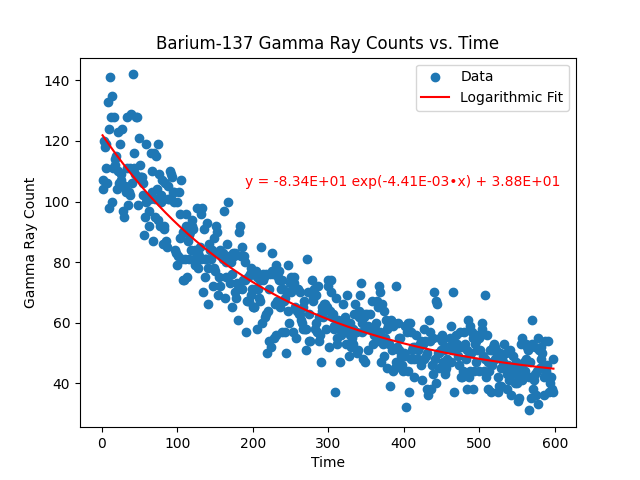
\includegraphics[width=.9\textwidth]{../images/day3_liquidtrial3_plot.png}
  \caption{A plot showing the exponential decays of our gamma ray counts, as plotted against time. .\label{fig:GammaRays} }
\end{figure}

\newpage





\section{Results}

The average half life we measured was $163.1 \pm 8.5$ seconds. This result 
is not totally consistent with the accepted result, but we are within one 
standard deviation of such result. As all of our trials also fell within this
range, we can state that we have observed the half life of Ba-137 correctly.


\section{Summary and Conclusions}

In this experiment, we observed the average half lifes of samples of Ba-137 to be 
$163.1 \pm 8.5$ seconds. This result is within one standard deviation of the accepted result.

I would like to thank my lab partner, Sannidhya Desai for his assistance on data
collection and overall assistance. Furthermore, I'd like to thank Dr. Dan Heinzen,
Parth Dave, and Konner Feldman for their assistance throughout the measurement and 
set up processes.


\begin{thebibliography}{9}
\bibitem{}D. C. Kweon, J. Choi, K.-R. Don, et al. “Use of a GM Counter to Measure
the Half-life of Ba-137m Generated by Using an Isotope Generator”. In:
Journal of the Korean Physical Society 65 (2014), pp. 532–540. url: https:
//link.springer.com/article/10.3938/jkps.65.532.
\bibitem{}Thaddeus J. Trenn. “Rutherford on the Alpha-Beta-Gamma Classifica-
tion of Radioactive Rays”. In: Isis 67.1 (1976), pp. 61–75. issn: 00211753,
15456994. url: http : / / www . jstor . org / stable / 231134 (visited on
09/16/2023).
\bibitem{}E. Henly and A. Garcia. Subatomic Physics. World Scientific, 2007.
\end{thebibliography}


\end{document}
